\section{Parallel Programmable Run-Time Monitoring}
\label{sec:monitoring}

\subsection{Overheads of Run-Time Monitoring}

% Previous work overheads
\begin{table*}[tb]
  \begin{center}
    \vspace{-0.0in}
    \begin{footnotesize}
    %\begin{tabular}{|l|p{2in}|r|r|}
\begin{tabular}{|l|l|l|r|}

\hline
{\bf Name} & {\bf Type} & {\bf Monitoring scheme and flexibility} & {\bf Slowdown (avg./worst)} \\ \hline\hline

DIFT \cite{dift-asplos04} & Custom HW & DIFT only & 1.1\% / 23\% \\ \hline
FlexiTaint \cite{flexitaint-hpca08} & Custom HW & DIFT w/ programmable policies & 1.1\%-3.7\% / 8.7\% \\ \hline
Hardbound \cite{hardbound-asplos08} & Custom HW & Array bounds checks only & 5\%-9\% / 22\% \\ \hline
Harmoni \cite{harmoni-dsn12} & Custom HW & Tag-based monitors & 1\%-10\% / 20\% \\ \hline\hline

FlexCore \cite{flexcore-micro10} & Dedicated FPGA & Instruction-trace monitoring & 1.05x-1.44x / 1.84x \\ \hline
FADE \cite{FIXME} & Core+Custom HW & Instruction-trace monitoring (effective when HW filters work) & \\ \hline
LBA-accelerated \cite{lba-isca08} & Multi-core+Custom HW & Instruction-trace monitoring (effective when accelerators work) & 1.02x-3.27x / 5x \\ \hline
LBA \cite{lba-asid06} & Multi-core+Custom HW & Instruction trace monitoring & 3.23x-7.80x / 11x \\ \hline \hline

Multi-core DIFT \cite{nagarajan-interact08} & SW (multithreaded) & DIFT (compiled for each application) & 1.48x / 2.2x \\ \hline

LIFT \cite{lift-micro06} & SW (DBI) & DIFT (fully flexible) & 3.6x / 7.9x \\ \hline
Purfiy \cite{purify-usenix92} & SW (DBI) & Memory leak checks (fully flexible) & 2.3x / 5.5x \\ \hline
TaintCheck \cite{taintcheck-05} & SW (DBI) & DIFT (fully flexible) & 10x / 27x \\ \hline


\end{tabular}

    \end{footnotesize}
    \caption{Overheads of various proposed run-time monitoring systems.}
    \vspace{-0.2in}
    \label{tab:monitoring.previous_overheads}
  \end{center}
\end{table*}

There have been numerous previous works exploring various implementations of
run-time monitoring systems. Table~\ref{tab:monitoring.previous_overheads}
summarizes some of these implementations and the average and worst-case
overheads reported. These systems vary in their hardware complexity,
flexibility, monitoring schemes, and overheads. Dedicated hardware can provide low 
overheads for specific monitoring schemes. However, more pronounced overheads are seen for 
flexible monitoring systems that implement monitoring on a processor core
\cite{lba-asid06, lba-isca08, nagarajan-interact08} or using an FPGA fabric
\cite{flexcore-micro10}. These systems allow a wide range of monitoring schemes to
be implemented on the same hardware architecture and also allow monitors to be modified and updated after deployment. However, in order to support this flexibility, they can easily incur tens of percent of
overhead in the average-case and severalfold slowdowns in the worst-case. Partial monitoring
can be a useful technique for reducing overheads for any of these systems.
In this paper, we will focus our discussion on using a parallel
processing core to implement the monitor. Our evaluation includes results
for both the core-based monitor as well as a higher performance FPGA-based monitor.

\subsection{Baseline Architecture}

% Run-time monitoring overview
\begin{figure}
  \begin{center}
    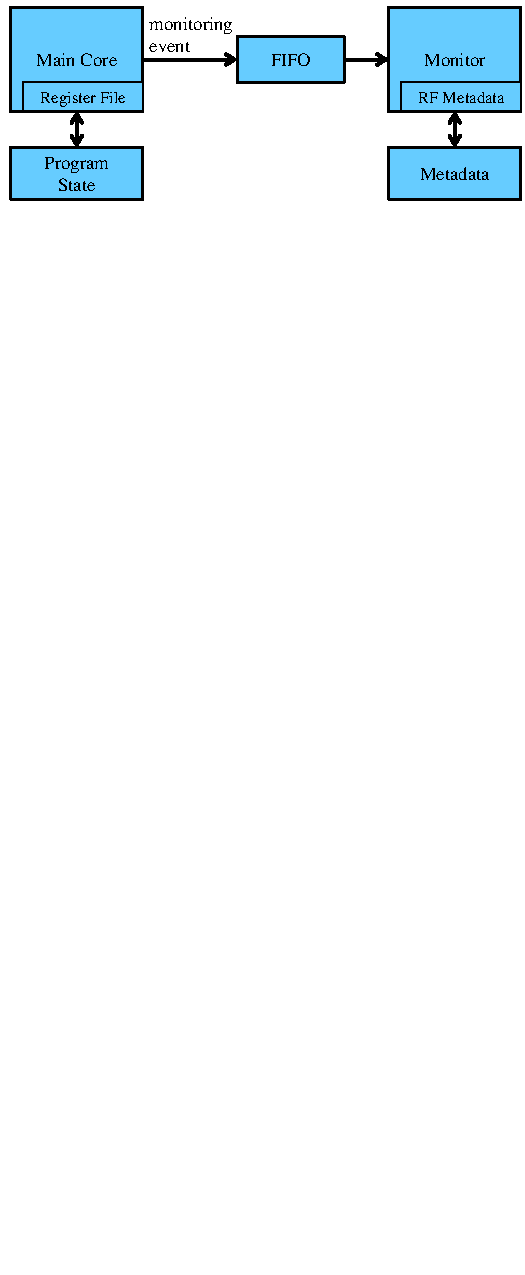
\includegraphics[width=\columnwidth]{figs/monitoring_architecture.pdf}
    \vspace{-0.2in}
    \caption{Overview of run-time monitoring architecture.}
    \label{fig:monitoring.overview} 
    \vspace{-0.1in}
  \end{center}
\end{figure}

Figure~\ref{fig:monitoring.overview} shows an overview of the run-time monitoring
model that is assumed in this paper.  The \emph{main program} is a computation
task that performs the original function of the system and is run on the
\emph{main core}.  On certain events during the main program, such as the
execution of certain types of instructions, the \emph{monitoring core} performs a
series of \emph{monitoring operations}. The monitoring core operates in parallel to the
main core. These events are referred to as \emph{monitoring events}. Depending
on the type of monitoring event, different monitoring operations are
executed. Information about monitoring events are sent to the monitoring core and buffered in a FIFO structure to decouple the
running of the main core and the monitoring core. If the FIFO is full, then the main
core is forced to stall on a monitoring event until a FIFO entry becomes
available. These stalls are a major source of
overhead because the monitoring core may take several cycles to process a single event
from the main core. We refer to these stalls and other overheads, such as
contention for shared resources, as \emph{monitoring overheads}. If the monitoring core
detects an inconsistent or undesired behavior in the monitoring events, then
an error is detected. 

There are many possible monitoring schemes that can be implemented on this type
of fine-grained parallel monitoring architecture such as memory protection
\cite{mondrian-asplos02}, information flow tracking \cite{dift-asplos04,
testudo-micro08}, soft error detection \cite{argus-micro07}, data-race
detection \cite{cord-hpca06}, etc.  For example, an array bounds check (BC)
\cite{hardbound-asplos08} can be implemented in order to detect
when software attempts to read or write to a memory location outside of an
array's bounds. This can be done by associating metadata with array pointers that 
indicates the array's base (start) and bound (end) addresses. On loads or stores with the
array
pointer, the monitoring core checks that the memory address accessed is within the base and
bound addresses. In addition, this base and bound metadata
is propagated on ALU and memory instructions to track the corresponding array pointers.
% One example is an uninitialized memory check (UMC) where monitoring is used to
% detect when software attempts to read from a memory location that was not
% previously initialized. This can be done by forwarding each load and store
% instruction from the main core to the monitor. For every memory location, the
% monitor keeps one bit of metadata. On a store to a memory location, the monitor
% marks the corresponding metadata bit to indicate that the memory location has
% been initialized. On a load, the monitor checks that the corresponding metadata
% bit has been previously marked as initialized.

% There are multiple options for implementing programmable parallel monitors. For
% example, the Log-Based Architecture \cite{lba-isca08} uses processor cores in a
% multi-core system as monitors. The FlexCore architecture
% \cite{flexcore-micro10} instead uses an FPGA-fabric to implement the
% monitor. 
% 
% The approach we describe in this paper applies to any of these
% parallel monitors. However, for experiments, we model an FPGA-based monitor
% similar to FlexCore.  The on-chip FPGA fabric is used to implement the
% ``Monitor'' block in Figure~\ref{fig:arch.overview} while the FIFO from the
% main core and metadata cache are implemented as ASICs.

% Example monitor
\begin{figure}
  \begin{center}
    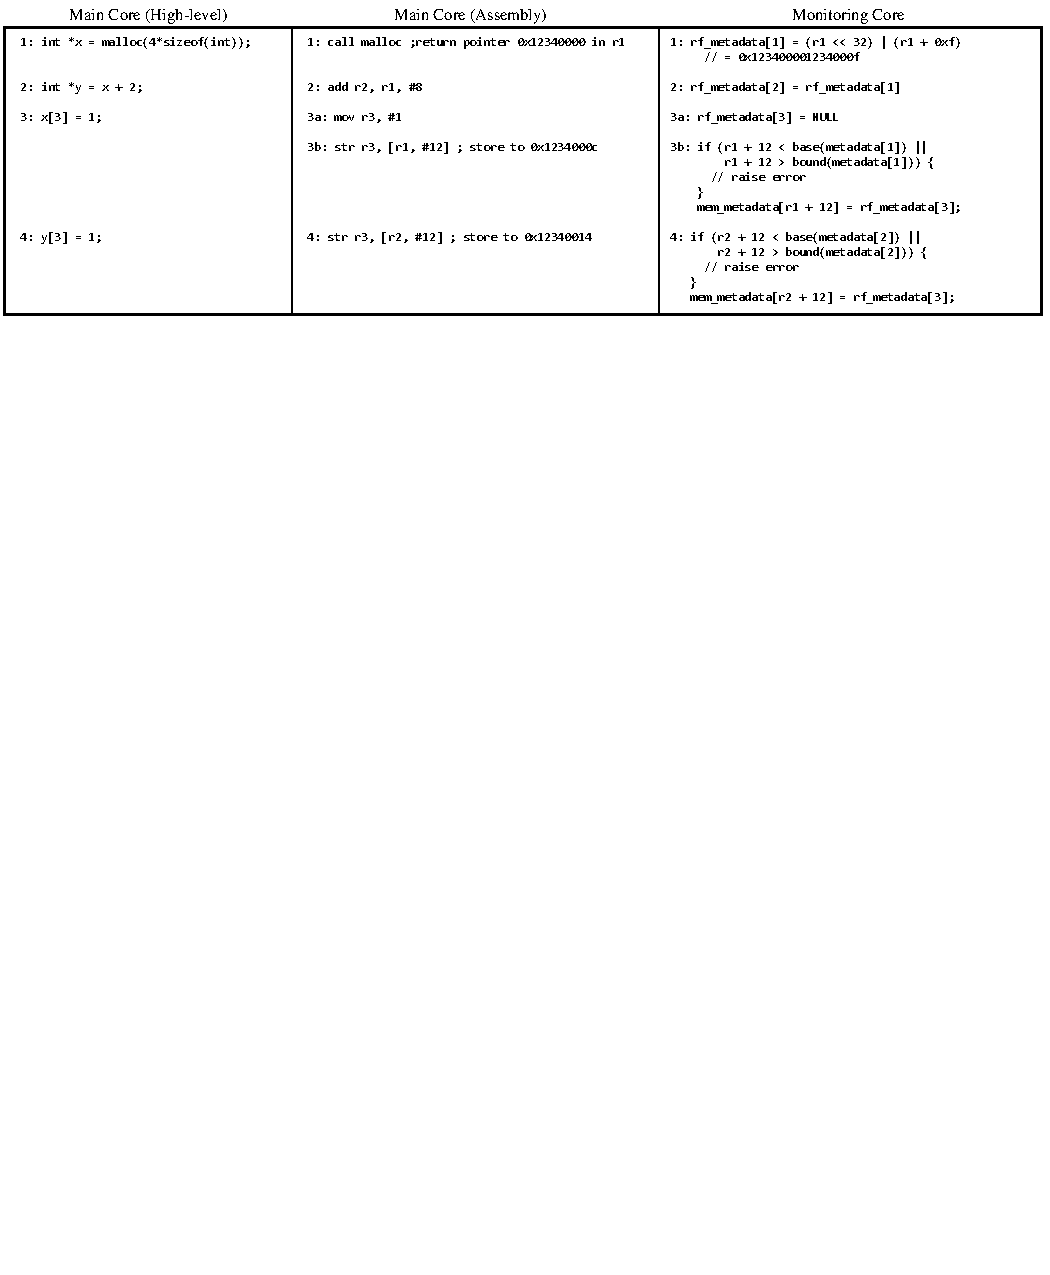
\includegraphics[width=\columnwidth]{figs/example_full.pdf}
    \vspace{-0.2in}
    \caption{Example of array bounds check monitor.}
    \label{fig:monitoring.example_full}
    \vspace{-0.1in}
  \end{center}
\end{figure} 

Figure~\ref{fig:monitoring.example_full} shows an example pseudo-code segment and
the corresponding monitoring operations for an array bounds check monitor. 
First, an array {\tt x} is allocated using {\tt malloc}. When this happens, the
monitor associates the array with metadata corresponding to its base and bounds
address. Next, {\tt y} is set to point to the middle of {\tt y}. The metadata
for {\tt y} is the same as the metadata {\tt x} to ensure that accesses using
{\tt y} do not exceed the bounds of {\tt x}. Finally, both pointers {\tt x} and
{\tt y} are used to perform a write. In both cases, the monitor checks whether
the address that is written to is within the bounds stored in the metadata. In
the first case, {\tt x+7} is within the original array's bounds. In the second
case, {\tt y+7} is not within the array's bounds and the monitor will raise an
error.


